\documentclass[a4paper,9pt]{extarticle}
\usepackage[utf8]{inputenc}
\usepackage[german]{babel}
\usepackage{multicol}
\usepackage{calc}
\usepackage{tikz}
\usepackage{polynom}
\usepackage{pifont}
\usepackage{amssymb}
\usepackage{setspace}

% noindent for paragraphs
\setlength\parindent{0pt}

% my packages:
\usepackage[landscape, left=0.75cm, top=1cm, right=0.75cm, bottom=1.5cm, footskip=15pt]{geometry}
\usepackage{amsmath, amssymb, amsfonts, amsthm, mathtools}
\usepackage{bbm}
\usepackage{tcolorbox}
\usepackage{enumitem}
\usepackage{physics}
\usepackage{extarrows}
\usepackage{algpseudocode}

% Turn off header and footer
\pagestyle{plain}

% Turn off page numbering
\pagenumbering{gobble}

% Tables
\usepackage{tabularx, multirow}
\usepackage{booktabs}
\renewcommand*{\arraystretch}{2}

% Make enumerations more compact
\usepackage{enumitem}
\setitemize{itemsep=0.5pt}
\setenumerate{itemsep=0.75pt}

% To include sketches
\usepackage{graphicx}

% Metadata
\title{\vspace{-1cm}Cheatsheet WuS\vspace{-0.65cm}}
\author{Amos Herz\vspace{-0.5cm}}
\date{FS 2021}

% remove spacing in lists and fancy enumerate
\usepackage{enumitem}
\setlist{noitemsep}

% change section/subsection/... font size
\usepackage{titlesec}
\titleformat*{\section}{\huge\bfseries}
\titleformat*{\subsection}{\large\bfseries}
% -----------------------------------------------------------------------

% a base set, that is then customised
\tcbset {
  base/.style={
    boxsep=1pt,left=1pt,right=3pt,top=3pt,bottom=3pt,
    boxrule=0mm,
    leftrule=1mm,
    left=1.75mm,
    arc=0mm, 
    fonttitle=\bfseries, 
    colbacktitle=black!10!white, 
    coltitle=black, 
    toptitle=0.75mm, 
    bottomtitle=0.25mm,
    title={#1}
  }
}

\definecolor{darkorange}{RGB}{255, 127, 0}
\definecolor{darkerorange}{RGB}{230, 114, 0}

\newtcolorbox{mainbox}[1]{
  colframe=darkorange, 
  base={#1},
}

\newtcolorbox{subbox}[1]{
  colframe=black!20!white,
  base={#1}
}

\tikzstyle{fancytitle} = [fill=darkerorange, text=white, font=\small\bfseries]

% Custom commands to make writing math easier
\newcommand\R{\mathbb{R}}
\newcommand\Q{\mathbb{Q}}
\newcommand\Z{\mathbb{Z}}
\newcommand\N{\mathbb{N}}
\newcommand\C{\mathbb{C}}
\newcommand\X{\mathcal{X}}
\newcommand\F{\mathcal{F}}
\newcommand\E{\mathbb{E}}
\newcommand\Pm{\mathbb{P}}
\newcommand\1{\mathbbm{1}}
\newcommand\Max{\mathrm{Max}}
\newcommand\Min{\mathrm{Min}}
\newcommand\Limit{\lim_{n \rightarrow \infty}}
\newcommand\Sup{\mathrm{Sup}}
\newcommand\Inf{\mathrm{Inf}}
\newcommand\Def{\textbf{Def.}\hspace{3mm}}
\newcommand\Bsp{\textit{Bsp.}\hspace{2mm}}
\newcommand\Satz{\textbf{{Satz.}}\hspace{3mm}}
\newcommand\Kor{\textbf{Kor.}\hspace{3mm}}
\newcommand\Bem{\textbf{Bem.}\hspace{3mm}}
\newcommand\converges[2]{\underset{#1\rightarrow #2}{\longrightarrow}}

\newcommand\Sum{\sum\limits}
\newcommand\Lim{\lim\limits}
\newcommand\Int{\int\limits}

\newcommand\Reihe{\sum_{k = 1}^{\infty}}

\newcommand*\diff{\mathop{}\!\mathrm{d}}

% Marked checkbox
\newcommand\marked{\rlap{\raisebox{0.3ex}{\hspace{0.4ex}\tiny \ding{52}}}$\square$}

% Custom Title
\newcommand\Title[1]{\vspace{1.5mm}\begin{tikzpicture} \node[fancytitle, right=10pt] {\textcolor{white}{#1}}; \end{tikzpicture}}

\begin{document}
\begin{multicols*}{3}

% _____ BEGINNING OF DOCUMENT __________________________________________________
\maketitle
\section*{Grundbegriffe}

Wir definieren einen \textbf{Wahrscheinlichkeitsraum} als das Tupel $(\Omega, \F, \Pm)$:

\begin{mainbox}{}
    Der \textbf{Grundraum} $\Omega$ ist eine nicht leere Menge, wobei $\omega \in \Omega$ ein Elementarereignis ist. \medskip
    
    Eine \textbf{Sigma-Algebra} $\F \subseteq \Pm(\Omega)$ erfüllt die Bedingungen:
    \begin{enumerate}
        \item $\Omega \in \F$
        \item $A \in \F \Rightarrow A^\complement \in \F$
        \item $A_1, A_2, ... \in \F \Rightarrow \bigcup^\infty_{i = 1} A_i \in \F$
    \end{enumerate} \medskip
    
    Ein \textbf{Wahrscheinlichkeitsmass} $\Pm$ auf $(\Omega, \F)$ ist eine Abbildung $\Pm : \F \mapsto [0,1], A \mapsto \Pm[A]$, so dass:
    \begin{enumerate}
        \item $\Pm[\Omega] = 1$
        \item $\Pm[A] = \sum_{i=1}^\infty \Pm[A_i]$, falls $A = \bigcup_{i = 1}^\infty A_i$
    \end{enumerate}
\end{mainbox}

Aus diesen Definitionen ergeben sich folgende nützliche Eigenschaften:
\begin{subbox}{}
\begin{enumerate}
    \item $\emptyset \in \F$
    \item $A_1, A_2, ... \in \F \Rightarrow \bigcap_{i = 1}^\infty A_i \in \F$
    \item $A, B \in \F \Rightarrow A \cup B \in \F$
    \item $A, B \in \F \Rightarrow A \cap B \in \F$
\end{enumerate}
\end{subbox}
und
\begin{subbox}{}
\begin{enumerate}
    \item $\Pm[\emptyset] = 0$
    \item $\Pm[A^\complement] = 1 - \Pm[A]$
    \item $\Pm[A \cup B] = \Pm[A] + \Pm[B] - \Pm[A \cap B]$
\end{enumerate}
\end{subbox}

Daraus ergibt sich, dass wenn $A_1, ..., A_n$ paarweise disjunkt sind: 
$$\Pm[A_1 \cup ... \cup A_n] = \Pm[A_1] + ... + \Pm[A_n]$$

\begin{mainbox}{\textbf{Monotonie}}
Seien $A, B \in \F$ dann gilt 
$$A \subseteq B \Rightarrow \Pm[A] \leq \Pm[B]$$
\end{mainbox}

\begin{mainbox}{\textbf{Union Bound}} Seien $A_1, A_2, ... \in \F$ dann gilt 
$$\Pm[\bigcup_{i = 1}^\infty A_i] \leq \sum_{i = 1}^\infty \Pm[A_i]$$
\end{mainbox}


\Title{Bedingte Wahrscheinlichkeiten}

Sei $(\Omega, \F, \Pm)$ ein Wahrscheinlichkeitsraum mit $A, B \in \F$ und $\Pm[B] > 0$. Die bedingte Wahrscheinlichkeit von $A$ gegeben $B$ ist definiert als:
$$\Pm[A | B] = \frac{\Pm[A \cap B]}{\Pm[B]}$$

\begin{mainbox}{\textbf{Totale Wahrscheinlichkeit}} Sei $A_1, ..., A_n \in \F$ eine Partition von $\Omega$ mit $\Pm[A_i] > 0$ für alle $1 \leq i \leq n$. Dann gilt:
$$\forall B \in \F. \quad \Pm[B] = \sum_{i = 1}^n \Pm[B | A_i] \cdot \Pm[A_i]$$
\end{mainbox}

\begin{mainbox}{\textbf{Formel von Bayes}} Sei $A_1, ..., A_n \in \F$ eine Partition von $\Omega$ mit $\Pm[A_i] > 0$ für alle $1 \leq i \leq n$. Für jedes $B \in \F$ mit $\Pm[B] > 0$ gilt:
$$\forall i = 1,...,n. \quad \Pm[A_i | B] = \frac{\Pm[B | A_i] \cdot \Pm[A_i]}{\sum_{k = 1}^n \Pm[B | A_k] \cdot \Pm[A_k]}$$
\end{mainbox}


\Title{Unabhängigkeit}

\begin{mainbox}{}
    Zwei Ereignisse $A, B \in \F$ sind \textbf{unabhängig} falls gilt:
    $$\Pm[A \cap B] = \Pm[A] \cdot \Pm[B]$$
\end{mainbox}

Daraus folgt, dass wenn $A \in \{0, 1\}$ zu jedem Ereignis $B$ unabhängig ist. Weiter gilt, wenn $A, B$ unabhängig sind, so müssen auch $A, B^\complement$ unabhängig sein. \medskip

Wir können Unabhängigkeit auch für mehr als zwei Ereignisse definieren. Seien $A_1, ..., A_n \in \F$, so sind die Ereignisse unabhängig falls gilt:
$$\forall I \subseteq \{1, ..., n\}. \quad \Pm[\bigcap_{i \in I} A_i] = \prod_{i \in I} \Pm[A_i]$$

\columnbreak
\section*{Zufallsvariablen}

Eine \textbf{Zufallsvariable} ist eine messbare Abbildung $X : \Omega \mapsto \R$, wobei $\Omega$ die Ereignismenge eines Wahrscheinlichkeitsraums $(\Omega, \F, \Pm)$ ist.
$$\forall x \in \R. \quad \{\omega \in \Omega \; | \; X(\omega) \leq x\} \in \F.$$
Hierbei schreiben wir oftmals nur $X$.


\Title{Verteilungsfunktion}

Die \textbf{Verteilungsfunktion} ist die Abbildung $F_X:\R \mapsto [0,1]$ definiert durch:
$$\forall x \in \R, \; F_X(x) = \Pm[X \leq x]$$

\begin{mainbox}{} Aus $a < b$ folgt:
$$\Pm[a < X \leq b] = F_X(b) - F_X(a)$$ \end{mainbox}

\begin{subbox}{Verteilungsfunktion Eingeschaften}
Die Verteilungsfunktion $F$ hat folgende Eigenschaften:
\begin{enumerate}
    \item $F$ ist monoton wachsend
    \item $F$ ist rechtsstetig, d.h. $\lim_{t \to 0} F(x + t) = F(x)$.
    \item $\lim_{x \to - \infty}F_X(x) = 0$ und $\lim_{x \to \infty}F_X(x) = 1$
\end{enumerate}
\end{subbox}

\Title{Unabhängigkeit von ZV}

\begin{mainbox}{Unabhängigkeit von ZV}
Die ZV $X_1,...,X_n$ sind unabhängig falls:
\begin{align*}
    \forall x_1,...,x_n \in \R. \quad &\Pm[X_1 \leq x_1, ..., X_n \leq x_n] \\ &= \Pm[X_1 \leq x_1] \cdot ... \cdot \Pm[X_n \leq x_n]
\end{align*}
\end{mainbox}

Eine Folge von Zufallsvariablen $X_1, X_2, ...$ ist:
\begin{enumerate}
    \item unabhängig, falls $\forall n. \quad  X_1,...,X_n$ unabhängig sind
    \item unabhängig und identisch verteilt (uiv.), falls sie unabhängig sind und $\forall i,j. \quad F_{X_i} = F_{X_j}$
\end{enumerate}


\Title{Transformation von ZV}

Sei $\varphi: \R \mapsto \R$ und $X$ ein Zufallsvariable, so ist 
$$\varphi(X) = \varphi \circ X$$ 
auch eine ZV. Seien $X_1,...X_n$ ZV mit $\phi: \R^n \mapsto \R$, so ist 
$$\phi(X_1, ..., X_n) = \phi \circ (X_1,...,X_n)$$
ebenfalls eine ZV.


%------------
% \columnbreak
%------------


\Title{Konstruktion einer ZV}

Sei eine gültige Verteilungsfunktion $F_X$ gegeben, nun wollen wir eine dazugehörige ZV $X$ konstruieren. Dafür brauchen wir: \medskip

\begin{mainbox}
    {Kolmogorov Theorem}
    $\exists (\Omega, \F, \Pm)$ und $\exists X_1, X_2, ... \text{ ZV in } (\Omega, \F, \Pm)$ sodass $X_1, X_2, ...$ uiv. Bernoullivariablen mit $p = 0.5$ sind.
\end{mainbox}

Sei $X_1, X_2,... \sim \text{Ber}(1/2)$ eine unendliche Folge, dann ist 
$$U = \sum_{n = 1}^\infty 2^{-n}\cdot X_n$$ 
gleichverteilt auf $[0,1]$. \medskip

Aufgrund der Eigenschaften der Verteilungsfunktion $F$, wissen wir dass eine eindeutige Inverse $F^{-1}$ existiert. wir können die generalisierte Inverse definieren als: 
\begin{subbox}{Die generalisierte Inverse}
$\forall \alpha \in [0,1]. \quad F^{-1}(\alpha) = \inf \{x \in \R \; | \; F(x) \geq \alpha\}$
\end{subbox}

Sei nun $F$ eine Verteilungsfunktion und $U$ eine gleichverteilte ZV in $[0,1]$. Dann besitzt $X = F^{-1}(U)$ genau die Verteilungsfunktion $F_X = F$. 
\section{Diskrete und Stetige ZV}

Per Definition ist eine Verteilungsfunktion immer rechtsstetig, analog dazu können wir die Linksstetigkeit definieren: 
$$F(x-) = \lim_{t \to 0} F(x-t)$$ 

Jedoch ist $F(x-) = F(x)$ nicht immer wahr, d.h. nicht jede Verteilungsfunktion ist linksstetig. \medskip

\begin{mainbox}{} $\forall x \in \R. \quad F(x) - F(x-) = \Pm[X = x]$.
\end{mainbox}
Daraus:
\begin{enumerate}
    \item Wenn $F$ in einem Punkt $a \in \R$ nicht stetig ist, dann ist die ``Sprünggrösse" $F(a) - F(a-)$ gleich der Wahrscheinlichkeit, dass $X = a$ ist.
    \item Wenn $F$ in einem Punkt $a \in \R$ stetig ist, dann ist $P[X = a] = 0$.
\end{enumerate}

\subsection{Fast sichere Ereignisse}

Ein Ereignis $A \in \F$ tritt \textbf{fast sicher} (f.s./a.s.) ein, falls $\Pm[A] = 1$. Seien $X,Y$ ZV, so schreiben wir: $X \leq Y$ f.s. $\Leftrightarrow \Pm[X \leq Y] = 1$.


\subsection{Diskrete ZV}

\begin{mainbox}{Diskret ZV}
    Eine ZV $X$ heisst \textbf{diskret}, falls $\exists W \subset \R$ endlich oder abzählbar, so dass $X \in W$ f.s. 
\end{mainbox}
\begin{subbox}{}
    Falls $\Omega$ endlich oder abzählbar ist, dann ist $X$ immer diskret.
\end{subbox}

\begin{mainbox}{}
Die \textbf{Verteilungsfunktion} einer diskreten ZV ist definiert als: 
$$(p(x))_{x \in W} \; \text{ wobei } \sum_{x \in W} p(x) = 1$$
\end{mainbox}
\begin{mainbox}{}
Die \textbf{Gewichtsfunktion} einer diskreten ZV ist definiert als: 
$$\forall x \in W. \quad p(x) = P[X = x]$$
\end{mainbox}

\subsection{Diskrete Verteilungen}

\subsection*{Bernoulli-Verteilung} 
Eine Bernoulli-Verteilte ZV kennt nur die Ereignisse $\{0,1\}$, wir schreiben auch $X \sim \text{Ber}(p)$. Sie wird definiert durch: 
\begin{mainbox}{Bernoulli-Verteilung}
    $$\Pm[X = 0] = 1 - p \; \text{ und } \; \Pm[X = 1] = p$$
\end{mainbox}

\subsection*{Binomialverteilung}
 Dies beschreibt die Wiederholung von Bernoulli-Experimenten. Wir schreiben $X \sim \text{Bin}(n,p)$ und definieren:

 \begin{mainbox}{Binomialverteilung}
    $$\forall k \in \{0, 1, ..., n\}. \quad \Pm[X = k] = \binom{n}{k} \cdot p^k \cdot (1-p)^{n-k}$$
 \end{mainbox}

 \begin{subbox}{}
    Sei $0 \leq p \leq 1, n \in \N$. \\
    Seien $X_1, \ldots , X_n$ unabhängige Bernoulli-Zufallsvariablen mit dem Parameter $p$. \\ Dann
    ist $S_n := X_1 + \ldots + X_n$
    eine binomial Zufallsvariable mit den Parametern $n$ und $p$.
\end{subbox}

Insbesondere ist die Verteilung Bin$(1, p)$ die gleiche wie die Verteilung Ber$(p)$. Man kann auch prüfen, dass wenn $X \sim$ Bin$(m, p)$ und $Y \sim$ Bin$(n, p)$ und $X, Y$ unabhängig sind, dann $X + Y \sim$ Bin$(m + n, p)$.

\subsection*{Geometrische Verteilung} Eine Geometrische Verteilung beschriebt das erste Auftreten eines Erfolges. Wir schreiben $X \sim \text{Geom}(p)$ und definieren:

\begin{mainbox}{Geometrische Verteilung}
    $$\forall k \in \N - \{0\}. \quad \Pm[X = k] = (1-p)^{k-1} \cdot p$$
\end{mainbox}

\begin{subbox}{}
    Sei $X_1, X_2, \ldots$ eine Folge von unendlich vielen unabhängigen Bernoulli ZV mit dem Parameter $p$. Dann
    $T := \text{min}\{n \geq 1 : X_n = 1\}$
    eine geometrische Zufallsvariable mit dem Parameter $p$.
\end{subbox}

\begin{subbox}{Abwesenheit der Erinnerung von der geometrische Verteilung}
    Sei $T \sim$ Geom$(p)$ für einige $0 < p < 1$. Dann
    $\forall n \geq 0 \forall k \geq 1 \Pm[T \geq n + k | T > n] = P[T \geq k]$.
\end{subbox}

\subsection*{Poisson-Verteilung} Diese Verteilung ist eine Annäherung an die Binomialverteilung für grosse $n$ und kleine $p$. Sie nimmt nur Werte in $\N$ an. Wir schreiben $X \sim \text{Poisson}(\lambda)$ und definieren:

\begin{mainbox}{Poisson-Verteilung}
    $$\forall k \in \N, \lambda > 0. \quad \Pm[X = k] = \frac{\lambda^k}{k!}\cdot e^{-\lambda}$$
\end{mainbox}

\begin{subbox}{Poisson-Approximation der Binomialform}
    Es sei $\lambda > 0$. Für jedes $n \geq 1$,
    betrachten wir eine Zufallsvariable $X_n \sim$ Bin$(n, \lambda / n)$. Dann
    $\forall k \in \N \lim_{n \rightarrow \infty} \Pm[X_n = k] = P[N = k]$,
    wobei $N$ eine Poisson-Zufallsvariable mit dem Parameter $\lambda$ ist.
\end{subbox}

\subsection{Stetige ZV}

\begin{mainbox}{}
    Eine ZV $X$ heisst \textbf{stetig}, wenn ihre Verteilungsfunktion $F_X$ wie folgt geschrieben werden kann:
    $$\forall x \in \R. \quad F_X(x) = \int_{-\infty}^x f(y)dy$$
\end{mainbox}

Hierbei ist $f: \R \mapsto \R_+$ die \textbf{Dichte} von $X$. Für die Dichte gilt:
$$\int_{-\infty}^{+\infty} f(y)dy = 1$$

Es gelten folgende Eigenschaften: 
\begin{enumerate}
    \item $\Pm [a \leq x \leq b] = \Pm [a < x < b]$ 
    \item $\Pm[X = x] = 0$
    \item $\Pm[X \in [a, b ]] = \Pm [X \in (a,b)]$
\end{enumerate}


\subsection{Stetige Verteilungen}

\subsection*{Gleichverteilung} 
Dies beschreibt die Situation wobei jedes Ereignis die gleiche Wahrscheinlichkeit hat. Wir schreiben $X \sim \mathcal{U}([a,b])$ und definieren:
\begin{mainbox}{Gleichverteilung}
$$f_{a,b}(x) = \begin{cases}
    0 & x \notin [a,b] \\
    \frac{1}{b-a} & x \in [a,b]
\end{cases}$$
\end{mainbox}
\begin{subbox}{Eigenschaften einer Gleichverteilte ZV $X$ in $[a, b]$:}
    \begin{itemize}
        \item Die Wahrscheinlichkeit, in ein Intervall $[c, c + l] \subset [a, b]$ zu fallen, hängt nur von seiner Länge $l$ ab:
        $$\Pm[X \in [c, c+l]] = \frac{l}{b-a}$$
        \item Die Verteilungsfunktion von $X$ ist gleich
        $$F_X(x) = \begin{cases}
            0 & x < a, \\
            \frac{x-a}{b-a} & a \leq x \leq b, \\
            1 & x > b.
        \end{cases}$$
    \end{itemize}
\end{subbox}

\subsection*{Exponentialverteilung} Dies ist das stetige Pendant zur Geometrischen Verteilung. Wir schreiben $X \sim \text{Exp}(\lambda)$ und definieren:
\begin{mainbox}{Exponentialverteilung}
    $$f_{a,b}(x) = \begin{cases}
        0 &x < 0 \\
       \lambda \cdot e^{-\lambda x} & x \geq 0
    \end{cases}$$
\end{mainbox}

\begin{subbox}{Eigenschaften einer Exponentialverteilte ZV $T$ mit Parameter $\lambda$}
    \begin{itemize}
        \item Die Wartezeitwahrscheinlichkeit ist exponentiell klein:
        $$\forall t \geq 0 \Pm[T > t] = e^{\lambda t}$$
        \item Abwesenheit der Erinnerung:
        $$\forall t, s\geq 0 \Pm[T > t + s|T > t] = \Pm[T > s]$$
    \end{itemize}
\end{subbox}


\subsection*{Normalverteilung} Wir schreiben $X \sim \mathcal{N}(m, \sigma^2)$ und definieren:
\begin{mainbox}{Normalverteilung}
    $$f_{m, \sigma}(x) = \frac{1}{\sqrt{2 \pi \sigma^2}} \cdot e^{-\frac{(x-m)^2}{2 \sigma^2}}$$
\end{mainbox}

\begin{subbox}{Eigenschaften einer Normalverteilte ZV}
    \begin{itemize}
        \item Wenn $X_1, \ldots , X_n$ sind unabhängige Zufallsvariablen mit Parametern $(m_1, \sigma^2_1), \ldots, (m_n, \sigma^2_n)$
        jeweils, dann
        $$Z = m_0 + \lambda_1X_1 + \ldots + \lambda_nX_n$$
        eine normale Zufallsvariable mit den Parametern $m = m_0 + \lambda_1m_1 + \ldots + \lambda_nm_n$ und $\sigma^2 = m_0 + \lambda^2_1\sigma^2_1 + \ldots + \lambda^2_n\sigma^2_n$ ist.
        \item Insbesondere, wenn $X \sim \mathcal{N}(0, 1)$ ist (in diesem Fall sagen wir, dass $X$ eine standardnormale
        Zufallsvariable), dann $$Z = m + \sigma \cdot X$$
        eine normale Zufallsvariable mit den Parametern $m$ und $\sigma^2$ ist.
        \item Wenn $X$ eine normale Zufallsvariable mit den Parametern $m$ und $\sigma^2$ ist, dann liegt die gesamte "Wahrscheinlichkeit
        Masse" hauptsächlich im Intervall $[m - 3\sigma, m + 3\sigma]$. Wir haben nämlich
        $$\Pm[ |X - m| \geq 3\sigma] \leq 0.0027$$
    \end{itemize}
\end{subbox}


\subsection*{Standard Normalverteilung} $\mathcal{N}(0,1)$. Weder für die zugehörige Dichte $\varphi(t)$ noch die Verteilungsfunktion $\Phi(t)$ gibt es geschlossene Ausdrücke, aber die Verteilung
\begin{mainbox}{Standard Normalverteilung}
    $$\Pm[X \leq t] = \Phi(t) = \int_{-\infty}^t \varphi(s)ds = \frac{1}{\sqrt{2 \pi}} \int_{-\infty}^t e^{-\frac{s^2}{2}}$$
\end{mainbox}


ist tabelliert. Ist $X \sim \mathcal{N}(\mu,\sigma^2)$, so ist $\frac{X - \mu}{\sigma} \sim \mathcal{N}(0,1)$.

\columnbreak
\section*{Erwartungswert}


Sei $X: \Omega \mapsto \R_+$ eine ZV mit nicht-negativen Werten. Dann ist 
$$\E[X] = \int_0^\infty (1 - F_X(x))dx$$
    
der \textbf{Erwartungswert} von $X$.


\Title{Erwartungswert diskreter ZV}

Sei $X: \Omega \mapsto \R$ eine diskrete ZV mit $X \in W$ f.s. Sei $\phi: \R \mapsto \R$ eine Abbildung. Falls die Summe wohldefiniert ist, gilt:
$$\E[\phi(X)] = \sum_{x \in W} \phi(x) \cdot \Pm[X = x]$$

Sei $\phi = \text{id}$, gilt 
$$\E[X] = \sum_{x \in W} x \cdot \Pm[X = x]$$


\Title{Erwartungswert stetiger ZV}

Sei $X$ eine stetige ZV mit Dichtefunktion $f$. Sei $\phi: \R \mapsto \R$ eine Abbildung, sodass $\phi(X)$ eine Zufallsvariable ist. Sofern das Integral wohldefiniert ist, gilt:
$$\E[\phi(X)] = \int_{-\infty}^\infty \phi(x)f(x)dx$$

 Auch hier können wir analog den Erwartungswert für $\phi = \text{id}$ definieren.


\Title{Rechnen mit Erwartungswerten}

\begin{mainbox}{}
    Seien $X,Y: \Omega \mapsto \R$ ZV mit $\lambda \in \R$. Falls die Erwartungswerte wohldefiniert sind, gilt:    
    $$\E[\lambda \cdot X + Y] = \lambda \cdot \E[X] + \E[Y]$$
    
    Wir nennen dies auch die \textbf{Linearität} des Erwartungswertes.
\end{mainbox}

Falls zwei ZV $X,Y$ \textbf{unabhängig} sind, dann gilt auch:
$$\E[X \cdot Y] = \E[X] \cdot \E[Y]$$

Dies gilt nicht für die Division, hier müssen wir wie folgt vorgehen
$$\E \Big[ \frac{X}{Y} \Big] = \E[X] \cdot \E \Big[ \frac{1}{Y} \Big]$$

und dabei $\E [1 / Y]$ individuell berechnen. Daraus ergibt sich dann die folgende Eigenschaft:

\begin{mainbox}{}
    Seien $X_1,...,X_n$ diskrete ZV. Dann sind die folgenden Aussagen äquivalent:
    \begin{enumerate}
        \item $X_1,...,X_n$ sind unabhängig
        \item Für jedes $\phi_1: \R \mapsto \R,..., \phi_n: \R \mapsto \R$ (messbar) beschränkt gilt:
        $$\E[\phi_1(X_1) \cdot ... \cdot \phi_n(X_n)] = \E[\phi_1(X_1)] \cdot ... \cdot \E[\phi_n(X_n)]$$
    \end{enumerate}
\end{mainbox}


\Title{Extremwertformel}

Sei $X$ eine diskrete ZV mit Werten in $\N$. Dann gilt folgende Identität, auch \textbf{Tailsum-Formel} genannt (\textbf{Achtung!} $n=1$):
$$\E[X] = \sum_{n=1}^\infty \Pm[X \geq n]$$

Sei $X$ eine stetige ZV mit $X \geq 0$ f.s., dann gilt:
$$\E[X] = \int_0^\infty \Pm[X > x] dx$$


\Title{Ungleichungen}

\begin{mainbox}{Monotonie} Seien $X,Y$ ZV sodass $X \leq Y$ f.s. dann gilt $\E[X] \leq \E[Y]$. \end{mainbox}

\begin{mainbox}
    {Markov Ungleichung} 
    
    Sei $X$ eine ZV mit $X \geq 0$ f.s. dann gilt für jedes $a > 0$:
    $$\Pm[X \geq a] \leq \frac{\E[X]}{a}$$
\end{mainbox}

\begin{mainbox}
    {Jensen Ungleichung} 
    
    Sei $X$ eine ZV und $\phi: \R \mapsto \R$ eine konvexe Funktion, dann gilt:
    $$\phi(\E[X]) \leq \E[\phi(X)]$$
\end{mainbox}


\Title{Varianz}

Sei $X$ eine ZV sodass $\E[X^2] < \infty$. Die \textbf{Varianz} von $X$ ist definiert durch 
\begin{mainbox}{Varianz}
   $$\text{Var}[X] = \sigma_X^2 = \E[(X-m)^2] = \E[X^2] - \E[X]^2$$ 
\end{mainbox}

wobei $m = \E[X]$. Dabei wird $\sigma_X$ auch die \textbf{Standardabweichung} von $X$ genannt und beschreibt die typische Distanz eines Wertes $x \in X$ zu $\E[X]$. \medskip

\begin{mainbox}
    {Chebychev Ungleichung}
    
    Sei $X$ eine ZV sodass $\E[X^2] < \infty$. Dann gilt für jedes $a \geq 0$:
    $$\Pm[|X - m| \geq a] \leq \frac{\sigma_X^2}{a^2}$$
\end{mainbox}

\begin{subbox}{}
    \begin{enumerate}
        \item Sei $X$ ein ZV sodass $\E[X^2] < \infty$ und $\lambda \in \R$: 
        $$\text{Var}[a \cdot X + b] = a^2 \cdot \text{Var}[X]$$
        \item $S = X_1 + ... + X_n$, wobei $X_1,...,X_n$ paarweise unabhängig sind, so gilt:
        $$\text{Var}[S] = \text{Var}[X_1] + ... + \text{Var}[X_n]$$
    \end{enumerate}
\end{subbox}


\Title{Kovarianz}

Die \textbf{Kovarianz} kann verwendet werden, um die Abhängigkeit zweier ZV zu messen.

\begin{mainbox}{Covarianz}
    Seien $X, Y$ zwei ZV mit $\E[X^2] < \infty, \E[Y^2] < \infty$, dann ist die \textbf{Kovarianz} zwischen $X, Y$ definiert als:
    $$\text{Cov}[X,Y] = \E[X \cdot Y] - \E[X] \cdot \E[Y]$$
\end{mainbox}
\section{Gemeinsame Verteilungen}


\subsection{Diskrete gemeinsame Verteilungen}

\begin{mainbox}{gemeinsame Verteilung}
    Seien $X_1,...,X_n$ diskrete ZV mit $X_i \in W_i$ f.s. für $W_i \subset \R$. Die \textbf{gemeinsame Verteilung} (GV) von $X_1,...,X_n$ ist die Familie $p = (p(x_1, ..., x_n))_{x_1 \in W_1, ..., x_n \in W_n}$ definiert durch:
    $$p(x_1, ..., x_n) = \Pm[X_1 = x_1, ..., X_n = x_n]$$
\end{mainbox}

Daraus ergibt sich folgende Eigenschaft. Sei $\phi: \R^n \mapsto \R$, so ist $Z = \phi(X_1,...,X_n)$ eine diskrete ZV mit Werten in $W = \phi(W_1 \cross ... \cross W_n)$ und folgender Verteilung:
$$\forall z \in W. \quad \Pm[Z = z] = \Sum_{ \substack{x_1 \in W_1, ... x_n \in W_n \\ \phi(x_1, ..., x_n) = z}} \Pm[X_1 = x_1, ..., X_n = x_n]$$

\begin{mainbox}{Randverteilung}
$$\forall z \in W_i.$$ $$\Pm[X_i = z] = \sum_{x_1, ..., x_{i-1}, x_{i+1},...,x_n} p(x_1, ..., x_{i-1}, z, x_{i+1},...,x_n)$$
\end{mainbox}

\begin{mainbox}
    {Erwartungswert}
    Der Erwartungswert definiert als:
$$\E[\phi(X_1, ..., X_n)] = \Sum_{x_1,...,x_n} \phi(x_1,...,x_n) \cdot p(x_1,...,x_n)$$
\end{mainbox} 

\Satz Folgenden Aussagen sind äquivalent:
\begin{enumerate}
    \item $X_1,...,X_n$ sind unabhängig
    \item Für alle $x_1 \in W_1, ..., x_n \in W_n$ gilt: 
    $$p(x_1,...,x_n) = \Pm[X_1 = x_1] \cdot ... \cdot \Pm[X_n = x_n]$$
\end{enumerate}


\subsection{Stetige gemeinsame Verteilungen}

\begin{mainbox}{gemeinsame Verteilung}
    Seien $X_1,...,X_n$ stetige ZV, so haben sie eine \textbf{gemeinsame Verteilung}, falls eine Funktion $f: \R^n \mapsto \R_+$ existiert, die für jedes $a_1,...,a_n \in \R$ folgende Eigenschaft erfüllt:
    $$\Pm[X_1 \leq a_1,..., X_n \leq a_n] = \int_{-\infty}^{a_1} ... \int_{-\infty}^{a_n} f(x_1,..., x_n) dx_n ... dx_1$$
    
    Wir nennen $f$ die \textbf{gemeinsame Dichte}.
\end{mainbox}

\begin{subbox}{} Seien $X_1,...,X_n$ stetige ZV mit einer gemeinsamen Dicht $f$ und $\phi: \R^n \mapsto \R$. Dann ist der Erwartungswert definiert als:
$$\E[\phi(X_1, ..., X_n)] = \int_{-\infty}^\infty ... \int_{-\infty}^\infty \phi(x_1, ...,x_n) \cdot f(x_1,...,x_n) dx_n...dx_1$$
\end{subbox}
\begin{subbox}{} Falls $X_1,...,X_n$ eine gemeinsame Dichte $f$ besitzt. Dann ist die Randverteilung:
\begin{align*}
    f_i(z) =& \int_{(x_1, ..., x_{i-1},x_{i+1},...x_n) \in R^{n-1}} \\ 
    & \quad f(x_1,...,x_{i-1},z,x_{i+1},...,x_n)dx_n...dx_{i+1}dx_{i-1}...dx_1
\end{align*}
\end{subbox}
\begin{subbox}{} Seien $X_1,...,X_n$ stetige ZV mit Dichten $f_1,..., f_n$, dann sind die folgenden Aussagen äquivalent:
\begin{enumerate}
    \item $X_1,...,X_n$ sind unabhängig
    
    \item $X_1,...,X_n$ sind stetig mit gemeinsamer Dichte: 
    $$f(x_1,...,x_n) = f_1(x_1) \cdot ... \cdot f_n(x_n)$$
    
    \item Für alle $\phi_1...,\phi_n : \R \mapsto \R$ gilt:
    $$\E[\phi_1(x_1) \cdot ... \cdot \phi_n(x_n)] = \E[\phi_1(x_1)] \cdot ... \cdot \E[\phi_n(x_n)]$$
\end{enumerate}\end{subbox}
\section*{Grenzwertsätze}

Gegeben eine unendliche Sequenz an uiv. ZV $X_1, X_2,...$, für jedes $n$ betrachten wir die Teilsumme $S_n = X_1 + ... + X_n$.

\begin{mainbox}
    {Gesetz der grossen Zahlen}
    
    Sei $\E[|X_1|] < \infty$ und $m = \E[X_1]$, so gilt:
    $$\lim_{n \to \infty} \frac{X_1 + ... + X_n}{n} = m \quad \text{f.s.}$$
\end{mainbox}

Da die ZV uiv. sind, gilt auch $\E[|X_i|] < \infty$ und $m = \E[X_i]$ für alle $i$. \medskip

\begin{subbox}{Konvergenz in Verteilung} Seien $(X_n)_{n \in \N}$ und $X$ ZV. Wir schreiben
$$X_n \approx X \quad \text{ für } n \to \infty$$

falls für jedes $x \in \R$ gilt:
$$\lim_{n \to \infty} \Pm[X_n \leq x] = \Pm[X \leq x]$$
\end{subbox}

\begin{mainbox}
    {Zentraler Grenzwertsatz}
    
    Sei $\E[X^2_1] < \infty$ und wohldefiniert. Weiter sei $m = \E[X_1]$ und $\sigma^2 = \text{Var}(X_1)$, so gilt:
    $$\Pm[ \frac{S_n - n \cdot m}{\sqrt{\sigma^2 \cdot n}} \leq a] \xlongrightarrow[n \to \infty]{} \Phi(a) = \frac{1}{\sqrt{2 \pi}} \int_{-\infty}^a e^{-x^2 / 2} dx$$
\end{mainbox}

Der Zentrale Grenzwertsatz besagt, dass die Verteilung einer ZV
$$Z_n = \frac{S_n - n \cdot m}{\sqrt{\sigma^2 \cdot n}}$$

wie die Verteilung von $\mathcal{N}(0,1)$ aussieht. Es gilt also
$$Z_n \approx Z \quad \text{ für } n \to \infty$$

wobei $Z \sim \mathcal{N}(0,1)$. Für normalverteilte ZV $X_1,...,X_n$, ist $Z_n$ immer Standardnormalverteilt.
\columnbreak
\section*{Sonstiges}

\begin{mainbox}{Summe Unhabhängiger ZV}
    $$f_{X+Y}(a) = \int_{y=-\infty}^{\infty} f_X(a - y)f_Y(y) dy$$
    \begin{align*}
        F_{X+Y}(a) & = \Pm(X+Y \leq a) \\
        & = \int \int_{x + y \leq a} f_X (x) f_Y(y) dx dy \\
        & = \int_{y = - \infty}^\infty \int_{x = -\infty}^{a - y} f_X(x) dx f_Y(y) dy \\
        & = \int_{y=-\infty}^{\infty} F_X(a - y)f_Y(y) dy
    \end{align*}
    Im Diskrete Falle, $\sum$ statt $\int$ und $p(y)$ statt $f(y)$
\end{mainbox}
\vfill\null
\columnbreak
\begin{center}
	\Large{\textbf{Statistik}}
\end{center}

\section*{Schätzer}

Wir nehmen an, dass wir wie einen Wahrscheinlichkeitsraum $(\Omega, \F, \Pm)$ und Zufallsvariablen $X_i$ haben. Zudem haben wir einen Parameterraum $\Theta \subset \R$, wobei $(\Pm_\theta)_{\theta \in \Theta}$ eine Familie von Wahrscheinlichkeitsmassen ist. $\Pm_\theta$ wird auch Modell genannt. Die Gesamtheit der beobachteten Daten nennen wir Stichprobe und die Anzahl $n$ den Stichprobenumfang.

\begin{mainbox}{Schätzer}
    Ein \textbf{Schätzer} ist eine Zufallsvariable $T: \Omega \mapsto \R$, von der Form:
    $$T = t(X_1,...,X_n), \quad t:\R^n \mapsto \R$$
\end{mainbox}

Ein Schätzer $T$ heisst \textbf{erwartungstreu} für den Modellparameter, falls für alle $\theta \in \Theta$ gilt:
$$\E_\theta[T] = \theta$$

Der \textbf{Bias} (erwarteter Schätzfehler) von $T$ im Modell $\Pm_\theta$ ist definiert als:
$$\E_\theta[T] - \theta$$

Der \textbf{mittlere quadratische Schätzfehler (MSE)} von $T$ im Modell $\Pm_\theta$ ist definiert als:
$$\text{MSE}_\theta[T] = \E_\theta[(T-\theta)^2]$$

$$\text{MSE}_\theta[T] = \text{Var}_\theta(T) + (\E_\theta[T] - \theta)^2$$


%------------
% \columnbreak
%------------



\Title{Maximum-Likelihood-Methode}

Nehmen wir an $X_1,...,X_n \in W$ sind ZV unter $\Pm_\theta$. Die \textbf{Likelikhood Funktion} ist definiert durch:
\begin{mainbox}{Likelikhood Funktion}
    $$L(x_1, ..., x_n; \theta) = \begin{cases}
        p(x_1, ..., x_n; \theta) & \text{im diskreten Fall} \\
        f(x_1, ..., x_n; \theta) & \text{im stetigen Fall} \\
        \end{cases}$$
\end{mainbox}

wobei $p$ respektive $f$ die gemeinsame Gewichtsfunktion / Dichtefunktion ist. Falls die $X_i$ uiv. sind unter $\Pm_\theta$, so gilt:
$$p_X(x_1,...,x_n;\theta) = \prod_{i=1}^n p_{X_i}(x_i; \theta)$$ $$f_X(x_1,...,x_n;\theta) = \prod_{i=1}^n f_{X_i}(x_i; \theta)$$

Für jedes $x_1, ..., x_n \in W$, sei $t_{\text{ML}}(x_1, ..., x_n)$ der Wert, der die Funktion $\theta \mapsto L(x_1, ..., x_n; \theta)$ maximiert. Ein \textbf{Maximum-Likelihood-Schätzer} ist definiert als: 
$$T_{\text{ML}} = t_{\text{ML}}(X_1,...,X_n)$$

Die \textbf{Log-Likelihood} Funktion hat den Vorteil, dass sie durch eine Summe anstelle eines Produkts gegeben ist und daher oftmals einfach zu berechnen ist.


\section*{Konfidenzintervalle}

Wir haben nun Methoden für Schätzer von unbekannten Parameter kennengelernt. Nun wollen wir wissen wie weit diese Schätzer vom effektiven Wert $p$ weg liegen.

\begin{mainbox}{Konfidenzintervall}
    Sei $\alpha \in [0,1]$. Ein \textbf{Konfidenzintervall} für $\theta$ mit Niveau $1 - \alpha$ ist ein Zufallsintervall $I = [A, B]$, sodass gilt 
    $$\forall \theta \in \Theta. \quad \Pm_\theta[A \leq \theta \leq B] \geq 1 - \alpha$$
    wobei $A,B$ ZV der Form $A = a (X_1, ..., X_n)$ und $B = b (X_1, ..., X_n)$, mit $a,b : \R^n \mapsto \R$, sind.
\end{mainbox}

Wenn wir nun einen $T = T_{\text{ML}} \sim \mathcal{N}(m, 1/n)$ haben, (dz.Bsp. $T_{\text{ML}}$ mit $X_1,...,X_n$ uiv. $\mathcal{N}(m, 1)$ oder $T = T_{ML} = \frac{X_1 + \ldots + X_n}{n}$) suchen wir einen Konfidenzinterfall der Form: 
$$I = [T - c/\sqrt{n}, T + c / \sqrt{n}]$$

Hierbei gilt:
\begin{align*}\Pm_\theta[T - c/\sqrt{n} \leq m \leq T + c/\sqrt{n}] &= \Pm_\theta[-c \leq Z \leq c] \\ &= \Pm_\theta[Z \leq c] - \Pm_\theta[Z < -c] \\ &= \Pm_\theta[Z \leq c] - (1 - \Pm_\theta[Z \leq c]) \\ &= 2\phi(c) - 1\end{align*}

wobei $Z = \sqrt{n}(T-m) =  \frac{X_1 + \ldots + X_n - mn}{\sqrt{n}}$ eine standardnormalverteilte ZV ist.

\renewcommand\arraystretch{1.8}
\begin{center}
    \begin{tabular}{c|c|p{4cm}|p{2.75cm}}
  		$\mu_0$ & $\sigma^2$ & Erwartungstreuer Schätzer & Verteilung under $\Pm_\theta$ \\
  		\hline
  		\hline
  		$\cross$ & $\checkmark$ & $\bar X_n = \frac{1}{n} \sum_{i=1}^n X_i$ & $\sqrt n (\frac{\bar X - \mu}{\sqrt \sigma^2}) \sim \mathcal{N}(0,1) $ \\
  		\hline
  		$\checkmark$ & $\cross$ & $T = \frac{1}{n} \sum_{i=1}^n (X_i - \mu)^2$ & $n \frac{T}{\sigma^2} \sim \mathcal{X}_n^2$ \\
  		\hline
  		$\cross$ & $\cross$ & $\mu: \bar X_n$, \medskip \newline $\sigma^2 : S^2 = \frac{1}{n-1} \sum_{i=1}^n(X_i - \bar X_n)^2$ & $ \sqrt n \frac{\bar X_n - \mu}{\sqrt S^2} \sim t_{n-1}$, \smallskip \newline $(n-1) \frac{S^2}{\sigma^2} \sim \mathcal{X}_{n-1}^2$ 
	\end{tabular}
\end{center}
\renewcommand{\arraystretch}{1}

\Title{Verteilungsaussagen}

\begin{mainbox}{{$\chi^2$-Verteilung}}
Eine stetige ZV heisst \textbf{$\chi^2$-verteilt} mit $m$ Freiheitsgrade, falls ihre Dichte gegeben ist durch
$$f_X(x) = \frac{1}{2^{\frac{m}{2}} \Gamma (\frac{m}{2})} x^{\frac{m}{2}-1} e^{-\frac{1}{2}x} \1_{x > 0},$$
\end{mainbox}
wobei 
$$\Gamma(v) = \int_0^\infty t^{v-1} e^{-t} dt.$$
Wir schreiben dann $X \sim \chi^2_m$.

Für natürliche Zahlen gilt $\Gamma(n) = (n-1)!$. Ein Spezialfall ist $m = 2$, hierbei erhalten wir $X \sim \text{Exp}(\frac{1}{2})$ \medskip

\begin{subbox}{} Für ZV $X_1, ..., X_m$ u.i.v. mit $X_i \sim \mathcal{N}(0,1)$ ist die Summe 
$$Y = \Sum_{i=1}^m X_i^2 \sim \chi_m^2$$
\end{subbox}
\begin{mainbox}{t-Verteilung}
Eine stetige ZV $X$ heisst \textbf{$t$-verteilt} mit $m$ Freiheitsgrade, falls ihre Dichte gegeben ist durch 
$$f_X(x) = \frac{\Gamma (\frac{m+1}{2})}{\sqrt{m \pi} \Gamma (\frac{m}{2})} \left( 1 + \frac{x^2}{m} \right)^{-\frac{m+1}{2}},$$
\end{mainbox}
\begin{subbox}{} Für $X, Y$ unabhängig mit $X \sim \mathcal{N}(0,1)$ und $Y \sim \chi^2_m$, ist der Quotient
$$Z = \frac{X}{\sqrt{\frac{Y}{m}}} \sim t_m.$$\end{subbox}


\Title{Normalverteilung mit $\mu, \sigma^2$ unbekannt }

\begin{subbox}{} Seien $X_1,...,X_n$ uiv. $\sim \mathcal{N}(\mu, \sigma^2)$. Dann sind
$$\overline{X}_n = \frac{1}{n} \Sum_{i=1}^n X_i \qquad \text{und} \qquad S^2 = \frac{1}{n-1} \Sum_{i = 1}^n (X_i - \overline{X}_n)^2$$
unabhängig. \end{subbox}

Nun haben wir $X_1,...,X_n$ ZV, die alle unter $\Pm_\theta$ uiv. $\sim \mathcal{N}(\mu, \sigma^2)$ sind. Die offensichtlichen Schätzer für $\mu, \sigma^2$ sind das Stichprobenmittel $\overline{X}_n$ und die Stichprobenvarianz $S^2$. Für jedes $\theta \in \Theta$ gilt:

$$\frac{\overline{X}_n - \mu}{S / \sqrt{n}} \sim t_{n-1} \text{ unter } \Pm_\theta$$

Also wollen wir:

$$1- \alpha \leq \Pm_\theta \left[ | \frac{\overline{X}_n - \mu}{S / \sqrt{n}} | \leq \frac{...}{ S / \sqrt{n}} \right]$$

Um eine kleines Intervall zu erhalten, wollen wir die Bedingung mit Gleichheit erfüllen und nehmen $\frac{...}{ S / \sqrt{n}} = t_{n-1, 1 - \alpha / 2}$, somit erhalten wir für $\mu$ folgendes Konfidenzintervall:

$$\left[ \overline{X}_n - t_{n-1, 1 - \alpha / 2} \frac{S}{\sqrt{n}},  \overline{X}_n + t_{n-1, 1 - \alpha / 2} \frac{S}{\sqrt{n}} \right]$$

Um ein Konfidenzintervall für $\sigma^2$ zu konstruieren brauchen wir:

$$\frac{1}{\sigma^2} (n-1) S^2 = \frac{1}{\sigma^2} \Sum_{i=1}^n (X_i - \overline{X}_n)^2 \sim \chi_{n-1}^2 \text{ unter } \Pm_\theta$$

Mit der Notation $\chi_{m, \gamma}^2$ für das $\gamma$-Quantil einer $\chi_m^2$ Verteilung wollen wir:

$$1 - \alpha = \Pm_\theta \left[ \chi_{n-1, \alpha/2}^2 \leq \frac{1}{\sigma^2} (n-1) S^2 \leq \chi_{n-1, 1- \alpha/2}^2\right]$$

Somit erhalten wir das Konfidenzintervall:

$$\left[ \frac{(n-1) S^2}{\chi_{n-1, 1-\alpha/2}^2} , \frac{(n-1) S^2}{\chi_{n-1, \alpha/2}^2} \right]$$

Fazit: Das wichtigste Tool zur Bestimmung von Konfidenzintervallen sind Verteilungsaussagen über Schätzer. Die ist im Allgemeinen aber schwierig / nicht möglich.


\Title{Approximative Konfidenzintervalle}

Zur Erinnerung der zentrale Grenzwertsatz besagt, dass wenn $X_i$ in $\Pm_\theta$ uiv. sind, dann ist $\sum_{i=1}^n X_i$ approximativ normalverteilt mit $\mu = n \E[X_i]$ und $\sigma^2 = n \text{Var}_\theta[X_i]$. Insbesondere können wir daraus auch eine standard normalverteilte ZV erhalten (siehe Grenzwertsatz).


\section*{Tests}


\Title{Null- und Alternativhypothese}

\begin{mainbox}{Null- und Alternativhypothese}
    Die \textbf{Nullhypothese $H_0$} und die \textbf{Alternativhypothese $H_A$} sind zwei Teilmengen $\Theta_0 \subseteq \Theta, \Theta_A \subseteq \Theta$ wobei $\Theta_0 \cap \Theta_A = \emptyset$. Eine Hypothese heisst \textbf{einfach}, falls die Teilmenge aus einem einzelnen Wert besteht; sonst zusammengesetzt.
\end{mainbox}


\Title{Test und Entscheidung}

\begin{mainbox}{Test}
    Ein \textbf{Test} ist ein $(T, K)$, wobei $T$ eine ZV der Form $T = t(X_1,...,X_n)$ ist und $K \subseteq \R$ ist eine deterministische Teilmenge von $\R$. Man nennt $T$ die \textbf{Teststatistik} und $K$ den \textbf{Verwerfungsbereich} oder kritischen Bereich.
\end{mainbox}

Wir wollen nun anhand der Daten $(X_1(\omega), ..., X_n(\omega))$ entscheiden ob die Nullhypothese akzeptiert oder verworfen wird. Dafür berechnen wir zuerst die Teststatistik $T(\omega) = t(X_1(\omega), ..., X_n(\omega))$ und gehen dann wie folgt vor:
\begin{itemize}
    \item die Hypothese $H_0$ wird verworfen, falls $T(\omega) \in K$
    \item die Hypothese $H_0$ wird nicht verworfen bzw. angenommen, falls $T(\omega) \notin K$
\end{itemize}

\begin{subbox}{Fehler 1. Art}
    Ein \textbf{Fehler 1. Art} ist, wenn die $H_0$ verworfen wird, obschon sie richtig ist.
    $$\Pm_\theta[T \in K], \quad \theta \in \Theta_0$$
\end{subbox}


\begin{subbox}{Fehler 2. Art}
    Ein \textbf{Fehler 2. Art} ist, wenn die $H_0$ akzeptiert wird, obschon sie falsch ist.
    $$\Pm_\theta[T \notin K] = 1 - \Pm_\theta [T \in K] \quad \theta \in \Theta_A$$

\end{subbox}


\Title{Signifikanzniveau und Macht}

Bei der Auswahl eines geeigneten Tests ist insbesondere die Minimierung von Fehlern 1. Art entscheidend. \smallskip

\begin{mainbox}{Signifikanzniveau}
    Sei $\alpha \in [0,1]$. Ein Test hat nun \textbf{Signifikanzniveau} $\alpha$ falls:
    $$\forall \theta \in \Theta_0. \quad \Pm_\theta[T \in K] \leq \alpha$$
\end{mainbox}

Das Sekundäre Ziel ist es den Fehler 2. Art zu vermeiden. \smallskip

\begin{mainbox}{Macht}
    Die \textbf{Macht} eines Tests wird definiert als Funktion:
    $$\beta: \Theta_A \mapsto [0,1], \quad \theta \mapsto \Pm_\theta[T \in K]$$
\end{mainbox}

\Bem $\alpha$ klein entspricht einer kleine Wahrscheinlichkeit für Fehler 1. Art, während $\beta$ gross einer kleinen Wahrscheinlichkeit für einen Fehler 2. Art entspricht. \smallskip

Das obige asymmetrische Vorgehen macht es schwieriger, die Nullhypothese zu verwerfen als sie beizubehalten. Ein guter Test wird deshalb als Nullhypothese immer die Negation der eigentlich gewünschten Aussage benutzen.

\Bem $\beta = 1 - \Pm_{H_A}[H_0 \text{ angenommen}]$. Das heisst, whenn zum Beispiel $\alpha = \Pm_{H_A}[T \leq 4]$ dann $\beta = 1 - \Pm[T > 4]$.

%------------
% \columnbreak
%------------



\Title{Konstruktion von Tests}

Wir nehmen an, dass $X_1,...,X_n$ diskret oder gemeinsam stetig sind unter $\Pm_{\theta_0}$ und $\Pm_{\theta_A}$, wobei $\theta_0 \neq \theta_A$ von der einfachen Form sind. \smallskip

\begin{subbox}{Likelihood-Quotient}
Der \textbf{Likelihood-Quotient} ist somit wohldefiniert:
$$R(x_1,...,x_n) = \frac{L(x_1,...,x_n; \theta_A)}{L(x_1,...,x_n; \theta_0)}$$
\end{subbox}

Wobei wir $R(x_1,...,x_n) = + \infty$ definieren falls $L(x_1,...,x_n; \theta_0) = 0$ sein sollte. Daraus ergibt sich, dass $R \gg 1 \Rightarrow H_A > H_0$ und $R \ll 1 \Rightarrow H_A < H_0$. \smallskip

\begin{mainbox}{Likelihood-Quotient-Test} 
    Sei $c \geq 0$. Der \textbf{Likelihood-Quotient-Test} (LQ-Test) mit Parameter $c$ ist definiert durch:
    $$ T = R(x_1,...,x_n) \quad \text{ und } \quad K = (c, \infty] $$
\end{mainbox}

Der LQ-Test ist optimal, da jeder andere Test mit einem kleineren Signifikanzniveau auch eine kleinere Macht hat:

\begin{mainbox}{Neyman-Paerson-Lemma}
    Sei $c \geq 0$ und $(T,K)$ der LQ-Test mit Parameter $c$ und $H_A = \theta_A, H_0 = \theta_0$.
$$\alpha^* = \Pm_{\theta_0}[T \in K]$$

Sei $(T', K')$ ein Test mit S-Niveau $\alpha \leq \alpha^*$ so gilt:
$$\Pm_{\theta_A}[T' \in K'] \leq \Pm_{\theta_A}[T \in K]$$
\end{mainbox}

\Title{p-Wert}

Wir wollen eine Hypothese $H_0 : \theta = \theta_0$ gegen eine Alternativhypothese $H_A : \theta \in \Theta_A$ testen. Eine Familie von Tests $(T, (K_t)_{t \geq 0})$ heisst \textbf{geordnet} bzgl. $T$ falls $K_t \subset \R$ und $s \leq t \Rightarrow K_t \subset K_s$ gilt. Typische Beispiele dafür sind $K_t = (t, \infty)$ (rechtsseitiger Test), $K_t = (-\infty, -t)$ (linksseitiger Test) und $K_t =  (-\infty, -t) \cup (t, \infty)$ (beidseitiger Test).

\begin{mainbox}{p-Wert}
    Sei $H_0: \theta = \theta_0$ eine einfache Nullhypothese und $(T, K_t)_{t \geq 0}$ eine geordnete Familie von Tests. Der \textbf{$p$-Wert} ist definiert als ZV $G(t)$, wobei:  
    $$G : \R_+ \mapsto [0,1], \quad G(t) = \Pm_{\theta_0}[T \in K_t]$$
\end{mainbox}

Der $p$-Wert hat folgende Eigenschaften:
\begin{subbox}{}
\begin{enumerate}
    \item Sei $T$ stetig und $K_t = (t, \infty)$, so ist der $p$-Wert unter $\Pm_{\theta_0}$ auf $[0,1]$ gleichverteilt.
    \item Für einen $p$-Wert $\gamma$ gilt, dass alle Tests mit Signifikanzniveau $\alpha > \gamma$ die Nullhypothese verwerfen.
\end{enumerate}
\end{subbox}

Wir können zusammenfassend sagen:
\begin{subbox}{}
    $$p\text{-Wert ist klein } \implies H_0 \text{ wird wahrscheinlich verworfen}$$
\end{subbox}


\subsection{Testbeispiele}
\subsubsection*{Normalverteilung, Test für Erwartungswert bei bekannter Varianz, z-Test}

\textbf{Variabeln}: $X_1, \ldots , X_n$ i.i.d. $\sim$ $\mathcal{N}(\theta, \sigma^2)$ unter $\Pm_\theta$ mit bekannter Varianz $\sigma^2$.

\textbf{Hypothese}: $H_0 : \theta = \theta_0$

\textbf{Alternativ}: $H_A : \theta > \theta_0$ oder $\theta < \theta_0$ (\textit{einseitig}), oder $\theta \neq \theta_0$ (\textit{zweiseitig}).

\textbf{Teststatistik}: $$T := \frac{\overline{X}_n - \theta_0}{\sigma / \sqrt{n}}$$

\textbf{Kritische Bereich}: $(c_>, \infty)$ wenn $H_A : \theta > \theta_0$, bzw. $(-\infty, c_<)$, bzw. $(-\infty, -c_\neq) \cup (c_\neq, \infty)$. Im zweiseitigen Fall verwirft man $H_0$ also zugunsten der Alternative $H_A : \theta \neq \theta_0$, falls $|T| > c_\neq$ ist.
Um $c_>, c_<, c_\neq$ zu bestimmen:
$$\alpha=\mathbb{P}_{\theta_{0}}\left[T \in K_{>}\right]=\mathbb{P}_{\theta_{0}}\left[T>c_{>}\right]=1-\mathbb{P}_{\theta_{0}}\left[T \leq c_{>}\right]=1-\Phi\left(c_{>}\right)$$ $$\Rightarrow c_> = \Phi^{-1}(1- \alpha) =: z_{1 - \alpha}$$
verwirft man also $H_{0}$, falls
$$
\overline{X}_{n}>\theta_{0}+z_{1-\alpha} \frac{\sigma}{\sqrt{n}}
$$
Analog ist $c_< = z_\alpha = -z_{1-\alpha}$ und $c_\neq z_{1 - \frac{\alpha}{2}}$.

\subsubsection*{Normalverteilung, Test für Erwartungswert bei unbekannter Varianz, t-Test}

\textbf{Variabeln}: $X_1, \ldots , X_n$ i.i.d. $\sim$ $\mathcal{N}(\theta, \sigma^2)$ unter $\Pm_\theta$ wobei $\theta = (\mu, \sigma^2)$.

\textbf{Hypothese}: $H_0 : \mu = \mu_0$

\textbf{Alternativ}: $H_A : \theta > \theta_0$ oder $\theta < \theta_0$ (\textit{einseitig}), oder $\theta \neq \theta_0$ (\textit{zweiseitig}).

\textbf{Teststatistik}:
$$
T:=\frac{\bar{X}_{n}-\mu_{0}}{S / \sqrt{n}} \sim t_{n-1} \text { unter } \mathbb{P}_{\theta_{0}}
$$
wir ersetzen also die unbekannte Varianz durch den Schätzer
$$
S^{2}=\frac{1}{n-1} \sum_{i=1}^{n}\left(X_{i}-\bar{X}_{n}\right)^{2}
$$

\textbf{Kritische Bereich}: die kritischen Werte hier sind $c_{>}=t_{n-1,1-\alpha}$, bzw. $c_{<}=t_{n-1, \alpha}=-t_{n-1,1-\alpha}$, bzw. $c_{f}=t_{n-1,1-\frac{\alpha}{2}}$. Für $t_{m, \gamma}$ es gilt $P\left[X \leq t_{m, \gamma}\right]=\gamma$ für $X$-verteilt mit $m$ Freiheitsgraden, d.h. $X \sim t_{m}$.

\subsubsection*{Gepaarter Zweistichproben-Test bei Normalverteilung}

\textbf{Variabeln}: $X_1, \ldots , X_n$ i.i.d. $\sim$ $\mathcal{N}(\mu_X, \sigma^2)$ und $Y_1, \ldots , Y_n$ i.i.d. $\sim$ $\mathcal{N}(\mu_Y, \sigma^2)$ unter $\Pm_\theta$ wobei $\theta = (\mu, \sigma^2)$.

Die Differenzen $Z_{i}:=X_{i}-Y_{i}$ sind nämlich unter $\mathbb{P}_{\theta}$ i.i.d. $\sim \mathcal{N}\left(\mu_{X}-\mu_{Y}, 2 \sigma^{2}\right)$. Damit kann man die bisherigen Tests in leicht angepasster Form benutzen, sowohl für bekannte wie für unbekannte Varianz $\sigma^{2}$. Die resultierenden Tests heissen dann nicht überraschend gepaarter Zweistichproben-z-Test (bei bekanntem $\left.\sigma^{2}\right)$ bzw. gepaarter Zweistichproben- $t$-Test (bei unbekanntem $\sigma^{2}$ ).

\subsubsection*{Ungepaarter Zweistichproben-Test bei Normalverteilung}

\textbf{Variabeln}: $X_1, \ldots , X_n$ i.i.d. $\sim$ $\mathcal{N}(\mu_X, \sigma^2)$ und $Y_1, \ldots , Y_m$ i.i.d. $\sim$ $\mathcal{N}(\mu_Y, \sigma^2)$ unter $\Pm_\theta$ wobei $\theta = (\mu, \sigma^2)$.
\begin{enumerate}
    \item $\sigma^{2}$ bekannt (\textit{ungepaarte Zweistichproben- $z$-Test.}): 

    \textbf{Teststatistik}:
    $$
    T:=\frac{\left(\bar{X}_{n}-\bar{Y}_{m}\right)-\left(\mu_{X}-\mu_{Y}\right)}{\sigma \sqrt{\frac{1}{n}+\frac{1}{m}}} \sim \mathcal{N}(0,1)
    $$
    unter jedem $\mathbb{P}_{\theta}$. Dabei ist $\sigma$ nach Annahme bekannt, und $\mu_{X}-\mu_{Y}$ muss sich aus der gewünschten Hypothese $H_{0}$ als bekannt ergeben. Die 
    
    \textbf{Kritischen Werte}: Wie oben geeignete Quantile der $\mathcal{N}(0,1)$-Verteilung, je nach Alternative. 
    \item $\sigma^{2}$ unbekannt \textit{Zweistichproben-t-Test}:
    
    $$
    \begin{aligned}
    &S_{X}^{2}:=\frac{1}{n-1} \sum_{i=1}^{n}\left(X_{i}-\bar{X}_{n}\right)^{2}, \\
    &S_{Y}^{2}:=\frac{1}{m-1} \sum_{j=1}^{m}\left(Y_{j}-\bar{Y}_{m}\right)^{2} .
    \end{aligned}
    $$
    Mit
    $$
    \begin{aligned}
    S^{2} &:=\frac{1}{m+n-2}\left((n-1) S_{X}^{2}+(m-1) S_{Y}^{2}\right) \\
    &=\frac{1}{m+n-2}\left(\sum_{i=1}^{n}\left(X_{i}-\bar{X}_{n}\right)^{2}+\sum_{j=1}^{m}\left(Y_{j}-\bar{Y}_{m}\right)^{2}\right)
    \end{aligned}
    $$
    ist dann die Teststatistik
    $$
    T:=\frac{\left(\bar{X}_{n}-\bar{Y}_{m}\right)-\left(\mu_{X}-\mu_{Y}\right)}{S \sqrt{\frac{1}{n}+\frac{1}{m}}} \sim t_{n+m-2}
    $$
    unter jedem $\mathbb{P}_{\theta}$. Der Rest geht dann analog wie oben.
\end{enumerate}
\section*{Sonstiges}


\Title{Nützliche Formeln}

$$ax^2 + bx + c = 0 \Rightarrow x = \frac{-b \pm \sqrt{b^2 - 4ac}}{2a}$$
$$\binom{n}{k} = \frac{n!}{(n-k)!k!}$$
$$\Sum_{k=0}^\infty q^k = \frac{1}{q	} \quad \text{für } |q| < 1$$
$$\Sum_{k=0}^n q^k = \frac{1 - q^{n+1}}{1 - q} \quad \text{für } q \neq 1$$
$$(x+y)^n = \sum_{k=0}^n \binom{n}{k} x^{n-k} y^k$$

%------------
% \columnbreak
%------------



\Title{Exponentialfunktion / Logarithmus}

Für die Exponentialfunktion gilt:
\begin{enumerate}[label = (\arabic*)]
	\item $\exp(x) \exp(y) = \exp(x+y)$
	\item $\exp(x) > 1, \quad \forall x > 0$
	\item $x^a = \exp(a \cdot \ln(x))$ und $x^0 = 1$
	\item $\exp(iz) = \cos(z) + i \cdot \sin(z)$
	\item $\exp(i \cdot \frac{\pi}{2}) = i$, $\exp(i \pi) = -1$ und $\exp(2 i \pi) = 1$
\end{enumerate}

Der natürliche Logarithmus $\ln : \, ]0, \infty[ \to \R$ bildet die Umkehrfunktion zu $\exp$ und ist
streng monoton wachsend und stetig. Für den natürliche Logarithmus gilt:

\begin{enumerate}[label = (\arabic*)]
	\item $\ln(1) = 0$
	\item $\ln(e) = 1$
	\item $\ln(a \cdot b) = \ln(a) + \ln(b)$
	\item $\ln(a / b) = \ln(a) - \ln(b)$
	\item $\ln(x^a) = a \cdot \ln(x)$
	\item $x^a \cdot x^b = x^{a + b}$
	\item $(x^a)^b = x^{a \cdot b}$
\end{enumerate}

Im Allgemeinen gilt $\log_b(a) = \frac{\ln(a)}{\ln(b)}$.


\Title{Ableitungs und Integrations Regeln}

\renewcommand\arraystretch{1.8}
\begin{center}
    \begin{tabular}{l|l}
        $F(x)$ & $F'(x) = f(x)$ \\
        \hline
        
        \textbf{Summenregel} & $(f(x) + g(x))' = f'(x) + g'(x)$ \\
		\textbf{Produktregel} & $(f(x) \cdot g(x))' = f'(x) \cdot g(x) + f(x) \cdot g'(x)$ \\
		\textbf{Quotientenregel} & $\left( \frac{f(x)}{g(x)} \right)' = \frac{f'(x) \cdot g(x) - f(x) \cdot g'(x)}{g^2(x)}$ wenn $g(x) \neq 0$ \\
		\textbf{Kettenregel} & $(f(g(x)))' = f'(g(x)) \cdot g'(x)$ \\
		\textbf{Part. Integration} & $\int f'(x) \cdot g(x) dx = f(x) \cdot g(x) - \int f(x) \cdot g'(x) dx$ \\
		\textbf{Substitution} & $\int_{\varphi(a)}^{\varphi(b)} f(x) \; dx = \int_a^b f(\varphi(t)) \cdot \varphi'(t) \; dt$ \\
		\textbf{Logarithmus} & $\int \frac{f'(t)}{f(t)} \; dt = \log(\abs{f(x)})$ \\
    \end{tabular}
\end{center}
\renewcommand{\arraystretch}{1}
  
\Bsp Substitution: Wir wollen $\int \cos(x^2) 2x \; dx$ berechnen dabei gehen wir wie folgt vor:

\begin{enumerate}
	\item Zuerst bestimmen wir die Substitution: $u = x^2$
	\item Nun berechnen wir die Umkehrfunktion: $x = \sqrt{u}$
	\item Dann brauchen wir noch: $\frac{du}{dx} = \frac{dx^2}{dx} = \frac{2x}{1} = 2x \implies dx = \frac{du}{2x}$
	\item Zuletzt können wir dies im Integral einsetzen und erhalten:
		$$\int \cos(x^2) 2x \; dx = \int \cos(u) 2x \; \frac{du}{2x} = \int \cos(u) \; du = \sin(u)$$
	
\end{enumerate}


\Title{Typische Ableitungen und Stammfunktionen}

\renewcommand\arraystretch{1.6}
\begin{center}
    \begin{tabular}{c|c}
        $F(x)$ & $F'(x) = f(x)$ \\
        \hline
            
        $ c $ & $ 0 $ \\
	    $ x^a $ & $ a \cdot x^{a - 1} $ \\
        $ \frac{1}{a+1} x^{a+1} $ & $ x^a $ \\
        $ \frac{1}{a\cdot(n+1)} (ax+b)^{n+1} $ & $ (ax+b)^n $ \\
	    $ \frac{x^{\alpha+1}}{\alpha + 1} $ & $ x^\alpha, \alpha \neq -1 $ \\
        $ \sqrt x $ & $ \frac{1}{2 \sqrt x} $ \\
        $ \sqrt[n] x $ & $ \frac{1}{n} {x}^{ \frac{1}{n} -1 } $ \\
        $ \frac{2}{3} x^{ \frac{3}{2} } $ & $ \sqrt x $ \\
        $ \frac{n}{n+1} x^{ \frac{1}{n}+1 } $ & $ \sqrt[n] x $ \\
	    $ e^x $ & $ e^x $ \\
	    $ \ln(|x|) $ & $ \frac{1}{x} $ \\
        $ \log_a |x| $  &  $ \frac{1}{x \ln a} = \log_a(e) \frac{1}{x} $ \\
        $ a^{cx} $ & $ a^{cx} \cdot c \ln a $ \\
        $ x^x $ & $ x^x \cdot (1+\ln x) \quad \scriptstyle x > 0 $ \\
        $ x \cdot (\ln |x| - 1) $  &  $ \ln |x| $ \\
    \end{tabular}
\end{center}
\renewcommand{\arraystretch}{1}


\Title{Funktionen}

\begin{center}
	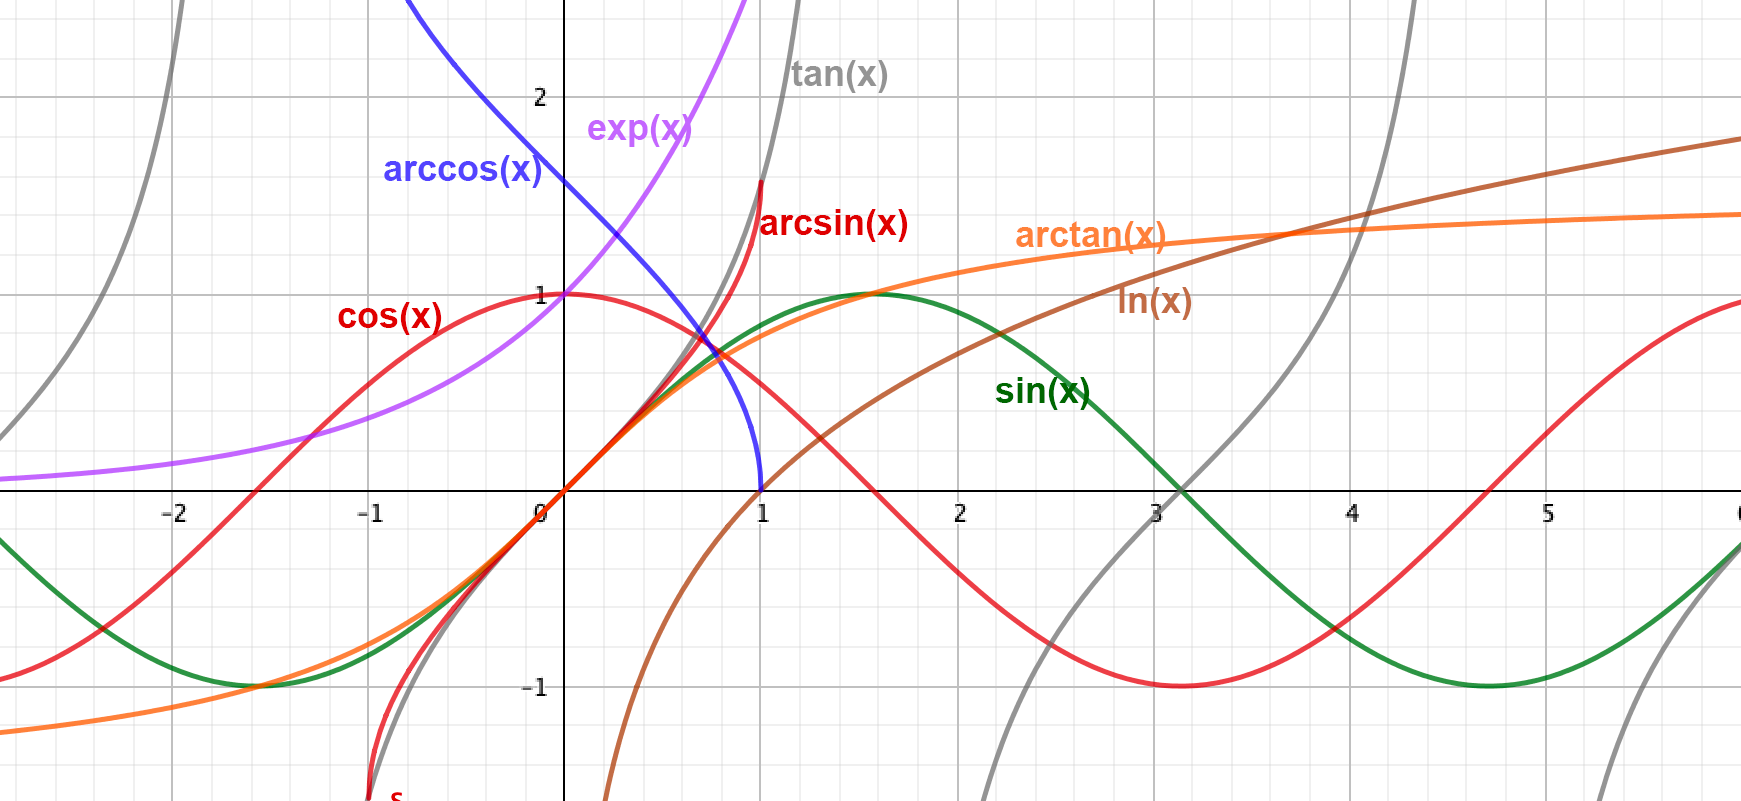
\includegraphics[width=\linewidth]{assets/funktionen.png}
\end{center}

\section{Aufgaben}


\subsection{Multiple Choice}

Seien $A_1, A_2, A_3 \in \F$ paarweise unabhängige Ereignisse, welche Aussage ist korrekt?
\begin{itemize}
	\item[\marked] Die Ereignisse $A_1, A_2, A_3$ sind nicht zwangsläufig unabhängig
	\item[$\square$] Die Ereignisse $A_1, A_2, A_3$ sind zwangsläufig unabhängig
\end{itemize}

\hrulefill

Es gilt $\Pm[X > t + s \; | \; X > s] = \Pm[X > t]$ für alle $t,s \geq 0$, falls
\begin{itemize}
	\item[$\square$] $X \sim \mathcal{U}([a,b])$
	\item[$\square$] $X \sim \text{Poisson}(\lambda)$
	\item[\marked] $X \sim \text{Exp}(\lambda)$ (Gedächnislosigkeit)
\end{itemize}

\hrulefill

Seien $X,Y$ zwei ZV mit gemeinsamer Dichte $f_{X,Y}$. Welche Aussage ist korrekt?
\begin{itemize}
	\item[\marked] $X,Y$ sind immer stetig
	\item[$\square$] Die ZV sind nicht notwendigerweise stetig.
\end{itemize}

\hrulefill

Seien $(X_i)_{i = 1}^n$ uiv. ZV mit Verteilungsfunktion $F_{X_i} = F$. Was ist die Verteilungsfunktion von $M = \text{max}(X_1,...,X_n)$?
\begin{itemize}
	\item[\marked] $F_M(a) = F(a)^n$
	\item[$\square$] $F_M(a) = 1 - F(a)^n$
	\item[$\square$] $F_M(a) = (1 - F(a))^n$
\end{itemize}

\subsection{Sonstige Aufgaben}

\textbf{Aufgabe}
Es werden ein blauer und ein grüner Würfel geworfen. Wir wählen $\Omega = \{1,...,6\}^2$. Wir betrachten die Algebra:
$$\F_{\text{sym}} = \{ A \subseteq \Omega \; | \; \forall (\omega_1, \omega_2) \in \Omega, (\omega_1, \omega_2) \in A \Leftrightarrow (\omega_2, \omega_1) \in A  \}$$
Zeige, dass $\F_{\text{sym}}$ eine $\sigma$-Algebra ist. \medskip

Wir müssen 3 Eigenschaften überprüfen. 
\begin{enumerate}
	\item $\forall (\omega_1, \omega_2) \in \Omega \Leftrightarrow (\omega_2, \omega_1) \in \Omega$ daher gilt $\Omega \in \F_{\text{sym}}$.
	\item Sei $A \in \F_{\text{sym}}$. Somit gilt für jedes $(\omega_1, \omega_2) \in \Omega$
		$$(\omega_1, \omega_2) \in A \Leftrightarrow (\omega_2, \omega_1) \in \Omega$$
		was äquivalent ist zu
		$$(\omega_1, \omega_2) \in A^\complement \Leftrightarrow (\omega_2, \omega_1) \in A^\complement$$
		somit ist $A^\complement \in \F_{\text{sym}}$.
	\item Seien $A_1, A_2, ... \in \F_{\text{sym}}$ gilt:
		\begin{align*}
			(\omega_1, \omega_2) \in \cup_{i=1}^\infty A_i &\Leftrightarrow \exists i. (\omega_1, \omega_2) \in A_i \\
			&\Leftrightarrow \exists i. (\omega_2, \omega_1) \in A_i \\
			&\Leftrightarrow (\omega_2, \omega_1) \in \cup_{i=1}^\infty A_i
		\end{align*}
		Somit folgt $\cup_{i=1}^\infty A_i \in \F_{\text{sym}}$.
\end{enumerate}

\hrulefill

\textbf{Aufgabe}
Sei $(X_i)_{i \geq 1}$ eine unendliche Folge von unabhängig $\text{Ber}(1/2)$-verteilten ZV. Wir betrachten folgenden Algorithmus:

\begin{algorithmic}
	\State $i \gets 1$
	\While{$X_i = X_{i+1}=1$}
		\State $i = i + 2$
	\EndWhile
	\State \Return $Z = X_i + 2 \cdot X_{i+1}$
\end{algorithmic}

Zeige, dass der Algorithmus immer nach endlich vielen Schritten terminiert (1). Zeige, dass $Z$ eine gleichverteilte ZV in $\{0,1,2\}$ ist (2). Konstruiert einen Algorithmus, der eine $\text{Ber}(1/5)$-verteilten ZV ausgibt (3). \medskip

(1) Wir definieren $A_j := \{ \text{While-Schlaufe wir j-Mal durchlaufen} \}$ und berechnen:
\begin{align*}
	\Pm[A_j] &= \Pm \left[ \bigcap_{i=1}^{2j} \{X_i = 1\} \cap (\{X_{2j+1} = 0\} \cup \{X_{2j+2} = 0\}) \right] \\
	&= \left( \Pi_{i=1}^{2j} \Pm[X_i = 1] \right) \cdot \Pm[X_{2j+1} = 0] \cdot \Pm[X_{2j+2} = 0] \\
	&= \left(\frac{1}{2}\right)^{2j} \cdot \frac{3}{4}
\end{align*}
Wenn wir nun über alle $A_j$ summieren, sehen wir, dass der Algorithmus immer in endlich Schritten terminieren wird. \medskip

(2) Wir wissen, dass alle $A_j$ disjunkt sind.
\begin{align*}
	\Pm[Z=0] &= \Pm[\{Z=0\} \cap A] + \Pm[\{Z=0\} \cap A^\complement] = \Sum_{j=0}^\infty \Pm[\{Z=0\} \cap A_j] \\
	&= \Sum_{j=0}^\infty \left(\frac{1}{2}\right)^{2j + 2} = \frac{1}{4}\Sum_{j=0}^\infty \left(\frac{1}{4}\right)^{j} = \frac{1}{4} \cdot \frac{1}{1 - \frac{1}{4}} = \frac{1}{3}
\end{align*}
Dies können wir nun auch für $1,2$ machen uns sehen, dass $Z$ gleichverteilt sein muss.

(3) Wir betrachten folgenden Algorithmus:
\begin{algorithmic}
	\State $i \gets 1$
	\While{$X_i = X_{i+2}=1 \text{ or } X_{i+1}=X_{i+2}=1$}
		\State $i = i + 3$
	\EndWhile
	\State \Return $Z = X_i + 2 \cdot X_{i+1} + 4 \cdot X_{i+2} = 4 \; ? \; 1 : 0$
\end{algorithmic}
Es ist leicht wie in $(1), (2)$ zu zeigen, dass er alle Eigenschaften erfüllt.

\hrulefill

\textbf{Aufgabe}
Sei $T \sim \text{Exp}(\lambda)$. Berechne die Dichte von $T' = c \cdot T^2$ und den Erwartungswert von $T'$. \medskip

Sei $\phi: \R \mapsto \R$ messbar und beschränkt. Wir definieren $\psi(x) = \phi(c \cdot x^2)$. Somit erhalten wir:
\begin{align*}
	\E[\phi(T')] &= \E[\phi(c \cdot T^2)] = \E[\psi(T)] = \int_{-\infty}^\infty \psi(x) \lambda e^{-\lambda x}\1_{x \geq 0}dx \\
	&= \int_0^\infty \phi(c \cdot x^2) \lambda e^{-\lambda x}dx = \int_0^\infty \phi(y) \lambda e^{-\lambda \sqrt{y / c}} \frac{dy}{2 \sqrt{cy}} \\
\end{align*}
Wobei wir die Dichte der Exponentialverteilung verwendet haben. daraus folgt:
$$f_{T'}(y) = \frac{\lambda}{2 \sqrt{cy}} e^{-\lambda \sqrt{y / c}}$$
Für den Erwartungswert gilt $\E[c \cdot T^2] = c \cdot \E[T^2]$:
$$\E[T^2] = \int_{0}^\infty x^2 \lambda e^{-\lambda x}dx = \frac{2}{\lambda^2}$$
Somit erhalten wir $\E[T'] = \frac{2c}{\lambda^2}$.

\hrulefill

\textbf{Aufgabe}
Sei $X$ eine ZV mit Verteilungsfunktion $F_X$. Zeige, dass $X$ diskret ist.
$$ F_X(a) = \begin{cases}
	0, 		& a < 1 \\
	1/5, 	& 1 \leq a < 4 \\
	3/4, 	& 4 \leq a < 6 \\
	1, 		& 6 \leq a \\
\end{cases}$$ \medskip

Wir stellen fest, dass $\Pm[X = x] = 0$ für alle $x \notin \{1,4,6\}$. Da die Menge $\{1,4,6\}$ endlich ist, ist die ZV diskret.

\hrulefill

\textbf{Aufgabe}
Sei $T$ eine ZV mit Verteilungsfunktion $F_T$. Zeige, dass $t$ stetig ist.
$$ F_T(a) = \begin{cases}
	0, 				& a < 0 \\
	1 - e^{-2a}, 	& a < \geq 0
\end{cases}$$ \medskip

Wir stellen fest, dass $F_T$ stückweise stetig differenzierbar ist (auf $(-\infty, 0)$ und $(0, \infty)$). Somit folgt, dass $T$ eine stetige ZV ist.




\end{multicols*}
\begin{small}
\section*{Diskrete Verteilungen}

\renewcommand{\arraystretch}{1.9}
\resizebox{\linewidth}{!}{
	\begin{tabular}{|c|p{3.3cm}|*{4}{c|}}
		\hline
		
		Verteilung & Parameter & $\mathbb{E}[X]$ & Var($X$) & $p_X(t)$ & $F_X(t)$ \\
		\hline
		
		Gleichverteilung & $n$: Anzahl Ereignisse \newline $x_i$: Ereignisse & $\frac{1}{n}\sum_{i=1}^{n}x_i$ & $\frac{1}{n}\sum_{i=1}^{n}x_i^2 -
		\frac{1}{n^2}\left(\sum_{i=1}^n x_i \right)^2$ & $\frac{1}{n}$ & $\frac{|\{k:x_k \leq t\}|}{n}$ \\
		\hline

		Bernoulli & $p$: ErfolgsWK & $p$ & $p \cdot (1-p) $ & $p^t(1-p)^{1-t}$ & $1-p$ für $0 \leq t < 1$ \\
		\hline

		Binomial & $p$: ErfolgsWK \newline $n$: Anzahl Versuche & $np$ & $np(1-p)$ & $\binom{n}{t}p^t(1-p)^{n-t}$ & $\sum_{k=0}^t\binom{n}{k}p^k(1-p)^{n-k}$ \\
		\hline

		Geometrisch & $p$: ErfolgsWK \newline $t$: Anzahl Versuche & $\frac{1}{p}$ & $\frac{1-p}{p^2}$ & $p(1-p)^{t-1}$ & $1-(1-p)^t$ \\
		\hline

		Poisson & $\lambda$: Erwartungswert \newline und Varianz & $\lambda$ & $\lambda$ & $\frac{\lambda^t}{t!}e^{-\lambda}$ & $e^{-\lambda} \Sum_{k=0}^{t} \frac{\lambda^k}{k!}$ \\
		\hline
	\end{tabular}
}


\section{Stetige Verteilungen}

\resizebox{\linewidth}{!}{
	\begin{tabular}{|c|p{2.8cm}|*{4}{c|}}
		\hline
		
		Verteilung & Parameter & $\mathbb{E}[X]$ & Var($X$) & $f_X(t)$ & $F_X(t)$ \\
		\hline

		Gleichverteilung & $[a,b]$: Intervall & $\frac{a+b}{2}$ & $\frac{1}{12}(b-a)^2$ & $\begin{cases}\frac{1}{b-a} & \text{for } t \in \{a, b\} \\ 0 & \text{otherwise}\end{cases}$ & $\begin{cases} 0 & \text{for } t < a \\ \frac{t-a}{b-a} & \text{for } t \in \{a, b\} \\ 1 \text{for } t > b \end{cases}$ \\
		\hline

		Exponentialverteilung & $\lambda: \frac{1}{\mathbb{E}[X]}$ & $\frac{1}{\lambda}$ & $\frac{1}{\lambda^2}$ & $\begin{cases} \lambda e^{-\lambda t}&t\geq 0\\0&t<0\end{cases}$ & $\begin{cases}1-e^{-\lambda t}&t>0\\0&t\leq 0\end{cases}$\\
		\hline

		Normalverteilung & $\sigma^2$: Varianz \newline $\mu: \mathbb{E}[X]$ & $\mu$ & $\sigma^2$ & \raisebox{-5pt}{$\frac {1}{\sqrt {2\pi \sigma^{2}}}e^{-{\frac {(t-\mu )^{2}}{2\sigma ^{2}}}} -\infty <t<\infty $} & \raisebox{-5pt}{${\frac {1}{\sigma {\sqrt {2\pi }}}}\int _{-\infty }^{t}e^{-{\frac{1}{2}}\left({\frac {y-\mu }{\sigma }}\right)^{2}}\mathrm {d} y$}\\
		\hline

		$\chi^2$-Verteilung & $n$: Freiheitsgrad & $n$ & $2n$ & $\frac{1}{2^{\frac {n}{2}}\Gamma ({\tfrac {n}{2}})}t^{{\frac {n}{2}}-1}e^{-{\frac {t}{2}}}\quad t>0$ & Gamma$(\frac{n}{2}, \frac{t}{2})$\\[8pt]
		\hline

		t-Verteilung & $n$: Freiheitsgrad & $\begin{cases} 0 & n > 1 \\ \text{undef.} & \text{sonst} \end{cases}$ & $\begin{cases} \frac{n}{n-2} & n > 2 \\ \infty & 1 < n \leq 2 \\ \text{undef.} & \text{sonst} \end{cases}$ & \raisebox{-2pt}{$\frac{\Gamma\left( \frac{n+1}{2}\right)}{\sqrt{n\pi} \cdot \Gamma(\frac{n}{2})} \left(1 + \frac{t^2}{n}\right)^{- \frac{n+1}{2}}$} & oof \\
		\hline
	\end{tabular}
}
\renewcommand{\arraystretch}{1}

\end{small}

% ____ FOOTER __________________________________________________________________
% Template:
% original by Christop Erdmann (erdmannc@student.ethz.ch), 2018
% modified by Andre Emmenegger, 2020
% modified by Danny Camenisch (dcamenisch@student.ethz.ch), 2021
% modified by Amos Herz (amherz@student.ethz.ch), 2021
%
% Content: 
% original by Amos Herz (amherz@student.ethz.ch), 2022
% based on different summaries from many helpful people

\end{document}